%\documentclass[12pt,a4paper,DIV12]{scrartcl}	% KOMASCRIPT :>
%\usepackage{fullpage}
\documentclass[12pt,a4paper,DIV12,twoside,parskip]{scrartcl}	% KOMASCRIPT :>
\usepackage{scrpage2}
\usepackage[ngerman]{babel}
\usepackage{lmodern}
\usepackage{mdwlist}
\usepackage[savepos]{zref}
\usepackage{refcount}
\usepackage{eurosym}
\usepackage{moresize}
\usepackage{needspace}
%\usepackage[cm]{fullpage}
\newlength{\border}
\newlength{\bcor}
\setlength{\border}{1.3cm}
\setlength{\bcor}{5mm}
%\usepackage[left=\border,top=1.5cm,right=\border,bottom=1.5cm]{geometry}
\usepackage[outer=\border,top=1.5cm,inner=1.8cm,bottom=1.5cm]{geometry}
%\usepackage[bottom=1cm,nohead,nofoot]{geometry}
%\usepackage[utf8]{inputenc}
\pagestyle{empty}
\usepackage{amsmath}
\usepackage{changepage}
\usepackage{color}
\usepackage{calc}
\usepackage{graphicx}
\usepackage{wallpaper}
\usepackage{everypage}
\usepackage{textcomp}
\usepackage{multicol}
\usepackage{eurosym}
\usepackage{wasysym}
\usepackage[absolute]{textpos}
%\usepackage[urw-garamond}{mathdesign}
%\usepackage{venturis}
\usepackage[T1]{fontenc}
\definecolor{tagcolor}{gray}{.4}
\newlength{\headwidth}
%\newlength{\haadheight}

\newcommand{\flushinner}{
\checkoddpage
\ifoddpage
\raggedright
\else
\raggedleft
\fi
}
\newcommand{\flushouter}{
\checkoddpage
\ifoddpage
\raggedleft
\else
\raggedright
\fi
}

\newcommand{\makebg}{
\genericbg
\checkoddpage
\ifoddpage
\ThisCenterWallPaper{1}{../linked/backgrounds/personenberichte-header-r.pdf}
\else
\ThisCenterWallPaper{1}{../linked/backgrounds/personenberichte-header-l.pdf}
\fi
}

\newlength{\rborder}

\newcommand{\setrborder}{
\checkoddpage
\ifoddpage
\setlength{\rborder}{\border+\bcor}
\else
\setlength{\rborder}{\border}
\fi
}

\newcommand{\genericbg}{
%\checkoddpage
%\ifoddpage
%\ThisCenterWallPaper{1}{../linked/backgrounds/background-r.pdf}
%\else
%\ThisCenterWallPaper{1}{../linked/backgrounds/background-l.pdf}
%\fi
}

\newcommand{\persontitle}[3]{
\setlength{\parindent}{0cm}
\settoheight{\headheight}{\titlefont \huge {#1}}
\begin{textblock*}{\textwidth}(\rborder,2cm-\headheight)
\flushouter
\textcolor{white}{\titlefont \huge {#1}}
\end{textblock*}
\settowidth{\headwidth}{\titlefont \huge {#1}}


\begin{textblock*}{\textwidth}(\rborder,2.2cm)
\flushouter
\parbox{\headwidth}{
\flushouter
\textcolor{white}{* \Dekar #2}
}
\end{textblock*}

\begin{textblock*}{\textwidth}(\rborder,2.2cm)
\flushouter
\parbox{\headwidth}{
\flushinner
\textcolor{white}{\Dekar #3}
}
\end{textblock*}
}

\newcommand{\personava}[1]{
\begin{textblock*}{\textwidth}(\rborder,8mm)
\flushinner
\parbox[top][5.2cm][b]{4.1cm}{\includegraphics[width=4.1cm]{#1}}
\end{textblock*}
}

\newcommand{\personmeta}[1]{
\begin{textblock*}{\textwidth}(\rborder,3.2cm)
\flushouter
\parbox{13cm}{
#1 \\
}
\end{textblock*}
}

\newcommand{\persontext}[4]{
\begin{textblock*}{\textwidth}(\rborder,6.7cm)
\flushouter
\large{#1}

%\vspace*{-1mm}
\small{\emph{#2}}\\
\end{textblock*}
\null
\begin{textblock*}{\textwidth}(\rborder,7.3cm)
%\parbox[top][17cm][t]{\textwidth}{
\setlength{\parindent}{5mm}
\begin{multicols}{2}
\noindent
#3
\end{multicols}
{#4}
%}
}

\newcommand{\hangpara}{
 \setlength{\parindent}{0cm} % don't indent new paragraphs
 \hangindent=0.4cm % indent all subsequent lines
}

\newcommand{\personauthorb}[1]{
\vspace*{-3mm}
\noindent
\parbox{\textwidth}{
\raggedleft
\it #1
}
\end{textblock*}
}
\newcommand{\persontagsb}[1]{
\begin{textblock*}{\textwidth}(\rborder,8.7cm)

\parbox[top][19.8cm][t]{\textwidth}{
\vspace{1em}
%\flushinner
%\sloppy
\scriptsize
\Slab
\textcolor{tagcolor}{\vfill #1}
}
\end{textblock*}
}

\newcommand{\makebgg}{
\checkoddpage
\ifoddpage
\ThisCenterWallPaper{1}{../linked/backgrounds/tplg-2.pdf}
\else
\ThisCenterWallPaper{1}{../linked/backgrounds/tplg-1.pdf}
\fi
}
\newcommand{\generichead}[1]{
\settoheight{\headheight}{\LARGE \Dekar {#1}}
\begin{textblock*}{\textwidth}(\border,8mm-\headheight)
\flushouter
\LARGE \Dekar \color{white} #1
\end{textblock*}
}

\newcounter{usegenericheaderc}
\setcounter{usegenericheaderc}{0}

\newcommand{\ghon}{\setcounter{usegenericheaderc}{1}}
\newcommand{\ghoff}{\setcounter{usegenericheaderc}{0}}

\newcommand{\generictitle}{f!xme}

\newcommand{\ornament}{
\vspace*{-8mm}
\begin{center}

\includegraphics[width=3cm]{ornament.pdf}
\end{center}
\vspace*{-2mm}
}

\newcommand{\say}[2]{
\parbox{\columnwidth}{
\hangindent=3mm
\textsc{\footnotesize #1} ,,{}#2{}``
\vspace*{1mm}
}
}

\newcommand{\saya}[3]{
\parbox{\columnwidth}{
\hangindent=3mm
\textsc{\footnotesize #1} \emph{\footnotesize #2} ,,{}#3{}``
\vspace*{1mm}
}
}

\newcommand{\sayn}[2]{
\parbox{\columnwidth}{
\hangindent=3mm
\textsc{#1} {}#2{}
\vspace*{1mm}
}
}

\newcommand{\newevenpage}{
\checkoddpage
\ifoddpage
\newpage
\else
\null
\fi
}

\newcommand{\studienfahrt}[2]{
\ghon
\renewcommand{\generictitle}{#1}
\newevenpage
\ThisCenterWallPaper{1}{../linked/backgrounds/bg2.pdf}
\begin{textblock*}{\paperwidth}(0cm,1.5cm)
\noindent
\includegraphics[width=\textwidth]{../photostack/#20.png}
\end{textblock*}
\null
\newpage
\ThisCenterWallPaper{1}{../linked/backgrounds/bg2.pdf}
\begin{textblock*}{\paperwidth}(0cm,1.5cm)
\noindent
\includegraphics[width=\textwidth]{../photostack/#21.png}
\end{textblock*}
}



\subsection*{$fach ${type}stündig bei $lehrer}
\addcontentsline{toc}{subsection}{$fach ${type}stündig bei $lehrer}
{\centering
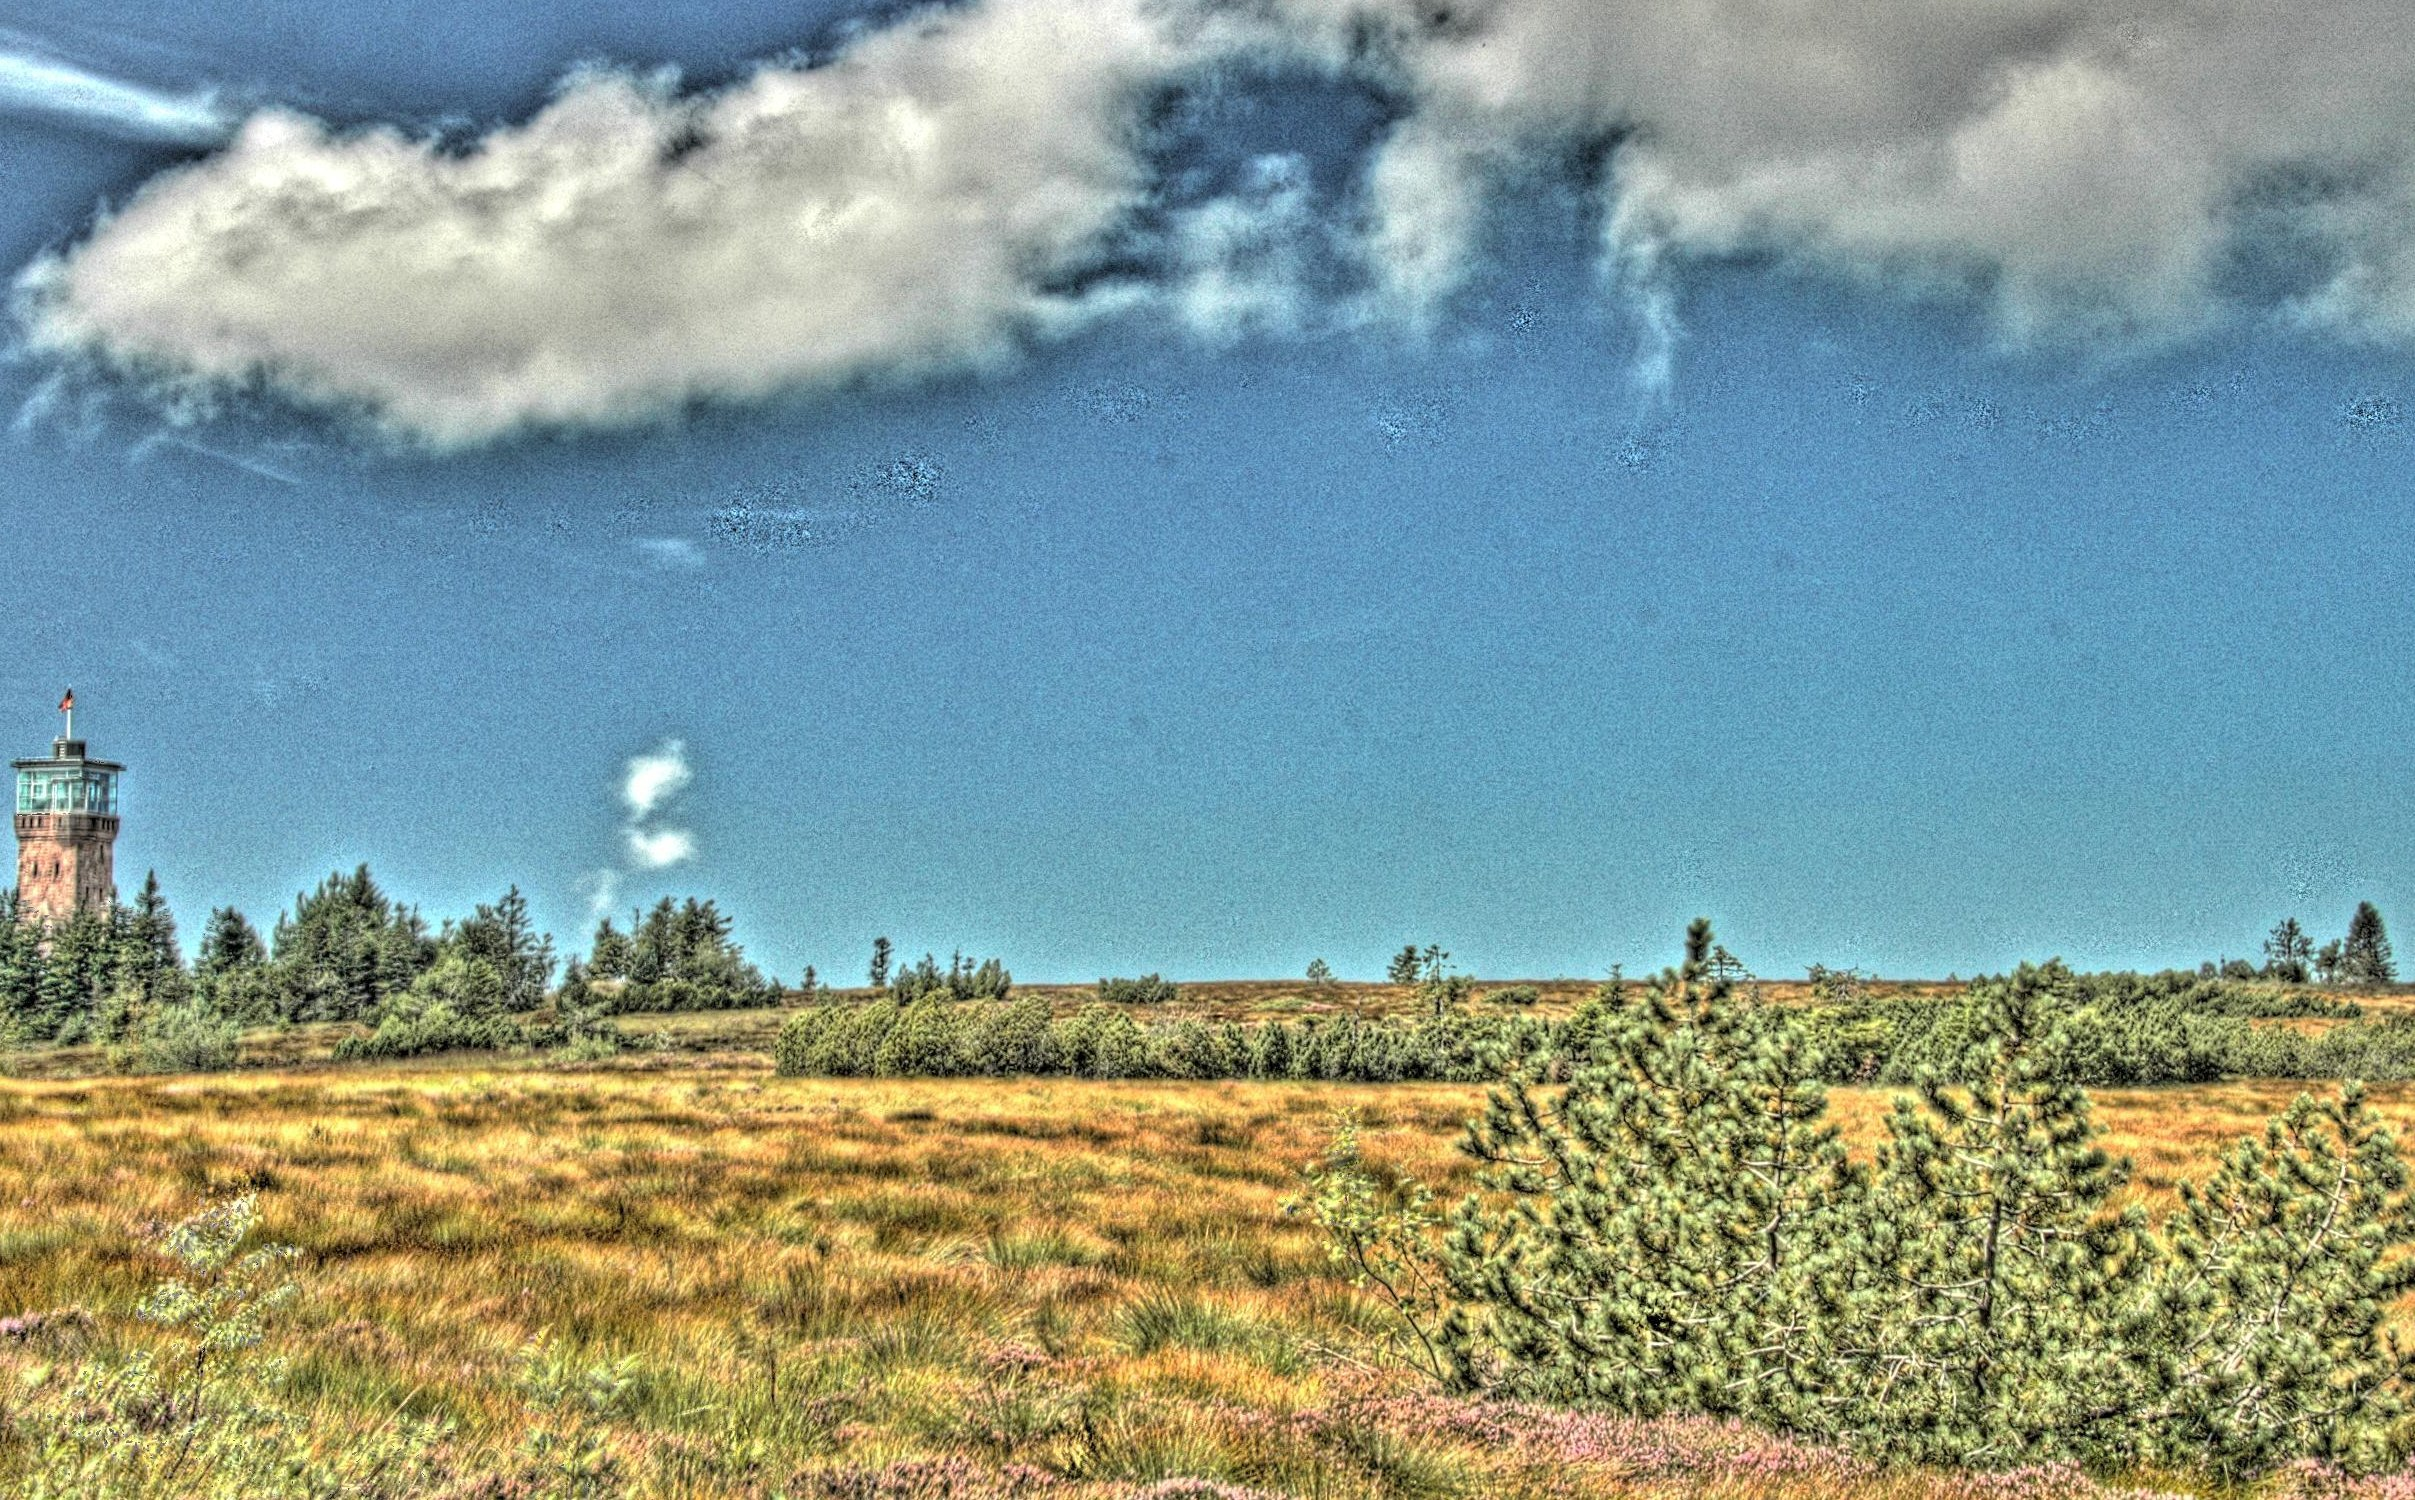
\includegraphics[width=\textwidth]{kurs.jpg}
}
%\vspace{5mm}
\\
$text

\vspace{3mm}
%\setlength{\parindent}{2cm}
{\em von $author}
\newpage

\parbox{\columnwidth}{
\noindent\begin{minipage}[top][5.4cm][c]{\columnwidth}\noindent\centering
\begin{tikzpicture}[scale=2]
\platzeins{#{name1}}{#{n1}}{#{ava1}}
\platzzwei{#{name2}}{#{n2}}{#{ava2}}
\platzdrei{#{name3}}{#{n3}}{#{ava3}}
\end{tikzpicture}\\
\vfill
\vspace*{-5mm} #{caption}
\end{minipage}
\vspace*{5mm}
}

%\setlength{\columnseprule}{0.2pt}
%\setlength{\columnsep}{30pt}
%\usepackage[compact]{titlesec}


\addtokomafont{subsubsection}{\rmfamily\normalsize}
\addtokomafont{subsection}{\rmfamily}
\usepackage[compact]{titlesec}
\titlespacing*{\subsubsection}{0pt}{*.5}{*.4}

%\titlespacing{\subsubsection}{0pt}{*1}{*0}
\usepackage{xltxtra}
\newfontfamily\titlefont[Scale=1.6]{Dekar}
\newfontfamily\Dekar{Dekar}
\newfontfamily\Slab{Museo Slab}
\newfontfamily\Tunga[Script=Kannada]{Tunga}
\newfontfamily\Fixed{Fixedsys Excelsior 3.01}
%\setmainfont{Museo Slab}
\newfontfamily\DjVu{DejaVu Sans}
\newfontfamily\FreeSerif{FreeSerif}
%\fontspec{/home/lukas/.fonts/HDZB_74.ttf}
\newfontfamily\Chinese{AR PL UMing CN}
%\lefoot{\Large\textcolor{white}{\Dekar \thepage \/ ABI WAN KENOBI}}
%\rofoot{\Large\textcolor{white}{\Dekar ABI WAN KENOBI \/ \thepage}}
\setlength{\parskip}{0mm}
\setlength{\footskip}{1.2cm}
\newcommand{\kathisize}{\fontsize{9.2pt}{11.04pt}\selectfont}
%\renewcommand{\subsubsectionheadstartvskip}{\vspace *{-1cm}}
\selectlanguage{ngerman}
\makeatletter
\let\rc@refused\refused
\makeatother

\usepackage{pdfpages}
%\usepackage{everyshi}
\begin{document}
\AddEverypageHook{{\ifnum\value{usegfc}=1 \makegbg \makefoot \else \makecontinuousfoot \fi} {\ifnum\value{usegenericheaderc}=1 \makebgg \generichead{\realtitle} \fi}}

\title{ABI WAN KENOBI}
\subtitle{\vspace{1cm}Möge G8 mit dir sein!}
\author{\vspace{2cm}}
\date{\Dekar Abitur 2012 am Fichte-Gymnasium Karlsruhe}
\maketitle
\thispagestyle{empty}
\newpage

\newcommand{\mychapter}[2]{
  \gfoff
  \renewcommand{\generictitle}{#2}
  \cleardoublepage
  \ThisCenterWallPaper{1}{../linked/backgrounds/chapters/{#1}.pdf}
  ~~
  \clearpage
  \gfon
}

\input{../linked/impressum.tex}
\newpage

\input{../linked/vorwort.tex}
\newpage

Inhaltsverzeichnis

\mychapter{1}{Die Padawane}
\includepdf[pages=2-20]{personenberichte.pdf}
\input{../linked/people/abgetretene.tex}

\mychapter{2}{Die Jedi-Akademien}
\includepdf[pages=2-20]{kursberichte.pdf}


\mychapter{3}{Imperial News}
%\renewcommand{\generictitle}{Memoiren}
\ghon
\renewcommand{\realtitle}{Memoiren}
\begin{multicols}{2}

\vspace{3mm}
{\raggedright Urbi et orbi. – Die Stadt und der Landkreis.}\\

\vspace{3mm}
{\raggedright ,,It’s the IGL’s! They have come to bring us wisdom!''}\\
\raggedleft \textsc{\footnotesize --\/Film}\\

\vspace{3mm}
{\raggedright ,,Ich stelle jetzt eine Erektionsgleichung auf…''}\\
\raggedleft \textsc{\footnotesize --\/Steffi}\\

\vspace{3mm}
\hangindent=0.7cm
\raggedright \textsc{\footnotesize Anna} ,,May I have your attention?''\\
\raggedleft ,,Immer!'' \textsc{\footnotesize Jonas}\\

\vspace{3mm}
\hangindent=0.7cm
\raggedright \textsc{\footnotesize Jonas} ,,Anna hat eh immer Recht.''\\
\raggedleft ,,Totale Monarchie hier!'' \textsc{\footnotesize Lucas}\\
\hangindent=0.7cm
\raggedright \textsc{\footnotesize Jonas} ,,Nein. \emph{Annarchie}!''\\

\vspace{3mm}
{\raggedright ,,Die Verbrechen der CDU sollten härter bestraft werden. Ähm. Die CDU will, dass Verbrechen härter bestraft werden.''}\\
\raggedleft \textsc{\footnotesize --\/Pia}\\

\vspace{3mm}
\hangindent=0.7cm
\raggedright \textsc{\footnotesize Kaindl} ,,Meine Tochter hat mal ein Stück Zeitung gegessen. Stirbt sie jetzt? Ich erzähle es euch...''\\
\raggedright \emph{\footnotesize (klingeln)}\\
\hangindent=0.7cm
\raggedright \textsc{\footnotesize Kaindl} ,,... nach der Pause.''\\

\vspace{3mm}
\hangindent=0.7cm
\raggedright \textsc{\footnotesize IGL} ,,How does the text convey its message?''\\
\raggedleft ,,Meybie wif samm rettorikell technieks?'' \textsc{\footnotesize David}\\

\vspace{3mm}
\hangindent=0.7cm
\raggedright \textsc{\footnotesize Kaindl} ,,Ist Glycogen löslich in Wasser?''\\
\raggedleft ,,Nö.'' \textsc{\footnotesize Fiz}\\
{\raggedright *pause*}\\
\hangindent=0.7cm
\raggedright \textsc{\footnotesize Fiz} ,,Glycogen ist nicht löslich in Wasser.''\\
\raggedleft ,,Ach soooo!'' \textsc{\footnotesize Kaindl}\\

\vspace{3mm}
\hangindent=0.7cm
\raggedright \textsc{\footnotesize Löhlein} ,,Der Luftwiderstand ist hier jetzt vernachlässigbar.''\\
\raggedleft ,,In Physik ist eigentlich alles vernachlässigbar...'' \textsc{\footnotesize Eglantine}\\

\vspace{3mm}
{\raggedright ,,Irgendwann heiratet Alex mal den Graphen von f.''}\\

\vspace{3mm}
\hangindent=0.7cm
\raggedright \textsc{\footnotesize Kaindl} ,,Das Symbol hat ein Herr Leibniz erfunden''\\
\raggedleft ,,...und direkt danach die Kekse.'' \textsc{\footnotesize Zeynep}\\

\vspace{3mm}
{\raggedright ,,Dünnschisschromatographie''}\\

\vspace{3mm}
\hangindent=0.7cm
\raggedright \textsc{\footnotesize Köhler} ,,Bitte beschreiben Sie das politische System der frühen USA.''\\
\raggedleft ,,Ich denke, das System wurde von den Gründerstaaten absichtlich stark kapitalistisch aufgebaut.'' \textsc{\footnotesize David}\\
\hangindent=0.7cm
\raggedright \textsc{\footnotesize Köhler} ,,Äh. Woran machen Sie das fest?''\\
\raggedleft ,,Hä? Woher soll ich denn wissen, woran die das festmachen... an der Wand?'' \textsc{\footnotesize David}\\

\vspace{3mm}
{\raggedright ,,Vielen Dank für diese Stellung.''}\\
\raggedleft \textsc{\footnotesize --\/Löhlein}\\

\vspace{3mm}
\hangindent=0.7cm
\raggedright \textsc{\footnotesize Nadine} ,,Jetzt schlagen Sie aber auch heftiger.''\\
\raggedleft ,,Genau, wie Ihr seht, schlage ich nicht mehr so stark.'' \textsc{\footnotesize Löhlein}\\

\vspace{3mm}
{\raggedright ,,ein Amoklauf - \emph{une promenade d'amok}''}\\

\vspace{3mm}
\raggedright \emph{\footnotesize (to) holler: \emph{v.} am Boden liegen; um Hilfe schreien}\\
\raggedleft \textsc{\footnotesize --\/Alex}\\

\vspace{3mm}
\hangindent=0.7cm
\raggedright \textsc{\footnotesize Karotke} ,,Charlotte, ist das ein Laser-Pointer?''\\
\raggedleft ,,Nein, das ist Lipgloss.'' \textsc{\footnotesize Charlotte}\\

\vspace{3mm}
{\raggedright ,,Ab 270 km/h zieht meine Gießkanne nach rechts.''}\\
\raggedleft \textsc{\footnotesize --\/Zeynep}\\

\vspace{3mm}
{\raggedright ,,Ja x hoch \emph{*räusper*} was da halt steht.''}\\
\raggedleft \textsc{\footnotesize --\/Passimü}\\

\vspace{3mm}
{\raggedright ,,Warum lustigt ihr?''}\\
\raggedleft \textsc{\footnotesize --\/Bohning}\\

\vspace{3mm}
{\raggedright ,,Man legt die Gleichung null.''}\\
\raggedleft \textsc{\footnotesize --\/Nadine}\\

\vspace{3mm}
\hangindent=0.7cm
\raggedright \textsc{\footnotesize  } ,,Herr Kaindls Tochter heißt Linnea.''\\
\raggedleft ,,Wieso hat er sie nicht ‚Parabella‘ genannt?'' \textsc{\footnotesize Seline}\\

\vspace{3mm}
{\raggedright ,,\emph{h} ausklammern... da geht einem das mathematische Herz auf.''}\\
\raggedleft \textsc{\footnotesize --\/Kaindl}\\

\vspace{3mm}
{\raggedright ,,Kommen Sie doch nicht immer von hinten.''}\\
\raggedleft \textsc{\footnotesize --\/Zeynep}\\

\vspace{3mm}
\hangindent=0.7cm
\raggedright \textsc{\footnotesize Kaindl} ,,Man sieht sich immer zweimal im Leben.''\\
\raggedleft ,,Wir sehen uns oft genug.'' \textsc{\footnotesize Zeynep}\\

\vspace{3mm}
\hangindent=0.7cm
\raggedright \textsc{\footnotesize Kunz} ,,Nenne zwei Amphibienarten.''\\
\raggedleft ,,Frösche und Enten.'' \textsc{\footnotesize Jonas}\\

\vspace{3mm}
{\raggedright ,,Ich hab mir mal mit einem Skalpell durch den \emph{ganzen} Finger geschnitten.''}\\
\raggedleft \textsc{\footnotesize --\/Fiz}\\

\vspace{3mm}
{\raggedright ,,Wir haben schon einige Parameter festgelegt, ihr wisst jetzt also, wo der Hase langläuft.''}\\
\raggedleft \textsc{\footnotesize --\/Hitz}\\

\vspace{3mm}
\hangindent=0.7cm
\raggedright \textsc{\footnotesize Pascal} ,,Also, wir können beobachten, dass das Pendel nach vorne und nach hinten schwingt.''\\
\raggedleft ,,Er meint: zur Seite...'' \textsc{\footnotesize Lucas}\\

\vspace{3mm}
{\raggedright ,,...das ist dann also die Vorstufe von Schimmel?''}\\
\raggedleft \textsc{\footnotesize --\/Nadine}\\

\vspace{3mm}
\hangindent=0.7cm
\raggedright \textsc{\footnotesize Köhler} ,,Wie funktionierten die ersten Eisenbahnen?''\\
\raggedleft ,,Mit Strom?'' \textsc{\footnotesize Nadine}\\
\hangindent=0.7cm
\raggedright \textsc{\footnotesize Köhler} ,,Nein. Strom gab es da noch nicht.''\\
\raggedleft ,,Hmm. Dann vielleicht .. Elektrizität?'' \textsc{\footnotesize Nadine}\\

\vspace{3mm}
\hangindent=0.7cm
\raggedright \textsc{\footnotesize Globas} ,,Das hier ist eine Blendsäule, und hier sieht man einen Pilaster.''\\
\raggedleft ,,Oooh!'' \textsc{\footnotesize Lucas}\\
\hangindent=0.7cm
\raggedright \textsc{\footnotesize Globas} ,,Jaahh ohh! Sexy Pilaster! Oooh!''\\

\vspace{3mm}
\hangindent=0.7cm
\raggedright \textsc{\footnotesize David} ,,Ist das jetzt richtig oder falsch?''\\
\raggedleft ,,Es ist richtig, dass es falsch ist!'' \textsc{\footnotesize Falko}\\

\vspace{3mm}
\hangindent=0.7cm
\raggedright \textsc{\footnotesize Löhlein} ,,So... auf der  Rückseite vom Blatt ist die Lösung ...''\\
\raggedright \emph{\footnotesize (alle drehen um)}\\
\hangindent=0.7cm
\raggedright \textsc{\footnotesize Löhlein} ,,... bei mir!''\\

\vspace{3mm}
{\raggedright ,,Ein Fehler, der oft falsch gemacht wird!''}\\
\raggedleft \textsc{\footnotesize --\/Schneider}\\

\vspace{3mm}
{\raggedright ,,Ich steh heute irgendwie auf der Leitung. Gut, dass ihr da seid!''}\\
\raggedleft \textsc{\footnotesize --\/Kaindl}\\

\vspace{3mm}
{\raggedright ,,Dürfen wir bei Ihnen mit offenem Mund gähnen?“''}\\
\raggedleft \textsc{\footnotesize --\/Maxi}\\

\vspace{3mm}
{\raggedright ,,Tipelditip''}\\
\raggedleft \textsc{\footnotesize --\/Kaindl}\\

\vspace{3mm}
{\raggedright ,,Jetzt bitte platzen.''}\\
\raggedleft \textsc{\footnotesize --\/Höll}\\

\vspace{3mm}
\hangindent=0.7cm
\raggedright \textsc{\footnotesize Nora Z.} ,,Der Witz mit dem Ständer ist nicht mehr lustig.''\\
\raggedleft ,,Ja, der ist ausgelutscht.'' \textsc{\footnotesize Luisa}\\

\vspace{3mm}
{\raggedright ,,Ist das 'ne Meldung oder ein schüchterner Stift?''}\\
\raggedleft \textsc{\footnotesize --\/Kaindl}\\

\vspace{3mm}
\hangindent=0.7cm
\raggedright \textsc{\footnotesize Kaindl} ,,Dann muss es schnaggeldischnack machen.''\\
\raggedright \emph{\footnotesize (Taschenrechner fällt auf den Boden)}\\
\hangindent=0.7cm
\raggedright \textsc{\footnotesize Kaindl} ,,Ja, so in etwa.''\\

\vspace{3mm}
\hangindent=0.7cm
\raggedright \textsc{\footnotesize Kaindl} ,,Und welche Einheit soll das jetzt haben?''\\
\raggedleft ,,Öhhhhm... Quadratgrad?'' \textsc{\footnotesize Jonas}\\

\vspace{3mm}
{\raggedright ,,Ich hab das jetzt nur gemacht, um die Zeit zu überbrücken.''}\\
\raggedleft \textsc{\footnotesize --\/Löhlein}\\

\vspace{3mm}
{\raggedright ,,Einmal ist keinmal.''}\\
\raggedleft \textsc{\footnotesize --\/Kunz}\\

\vspace{3mm}
{\raggedright ,,Krossing-Öiver''}\\
\raggedleft \textsc{\footnotesize --\/Kunz}\\

\vspace{3mm}
\hangindent=0.7cm
\raggedright \textsc{\footnotesize Zeynep} ,,Also an ihrer Stelle würde ich keine Gruppenarbeiten mehr anordnen, Sie langweilen sich immer so.''\\
\raggedleft ,,Joa, schon so.'' \textsc{\footnotesize Kaindl}\\
\hangindent=0.7cm
\raggedright \textsc{\footnotesize Seline} ,,(plötzlich) Spielen Sie doch ein Spiel.''\\

\vspace{3mm}
\hangindent=0.7cm
\raggedright \textsc{\footnotesize Hitz} ,,Kerim? Hast du gerade eine Bastelstunde eröffnet?''\\
\raggedleft ,,Nein. Er hat sein Mäppchen aufgemacht.'' \textsc{\footnotesize Jonas}\\

\vspace{3mm}
{\raggedright ,,Never ever don’t do that, \emph{ne pas faire quelque chose comme ca} - auf Spanisch kann ichs nicht... hola, hola!''}\\
\raggedleft \textsc{\footnotesize --\/Kaindl}\\

\vspace{3mm}
\hangindent=0.7cm
\raggedright \textsc{\footnotesize Wittorski} ,,Welches Kind wird häufig bei den Römern dargestellt, so um 53 v. Christus?''\\
\raggedleft ,,Jesus.'' \textsc{\footnotesize  }\\

\vspace{3mm}
{\raggedright ,,Das muss verstanden worden sein.''}\\
\raggedleft \textsc{\footnotesize --\/Kunz}\\

\vspace{3mm}
{\raggedright ,,Goethe, Schiller und Lessing waren damals genau gleich alt, außer Goethe, der war älter.''}\\
\raggedleft \textsc{\footnotesize --\/Hitz}\\

\vspace{3mm}
{\raggedright ,,Ich geh' langsam aus dem Kleister.''}\\
\raggedleft \textsc{\footnotesize --\/Hitz}\\

\vspace{3mm}
{\raggedright ,,Falsch ist aber auch nicht richtig.''}\\
\raggedleft \textsc{\footnotesize --\/Hitz}\\

\vspace{3mm}
{\raggedright ,,Ein Balkon, zwei Balkan.''}\\
\raggedleft \textsc{\footnotesize --\/Zeynep}\\

\vspace{3mm}
\hangindent=0.7cm
\raggedright \textsc{\footnotesize  } ,,Was passiert, wenn ein Minderjähriger eine Minderjährige sexuell belästigt?,,''\\
\raggedleft ,,Faaaaaalkooooo!'' \textsc{\footnotesize Lucas}\\

\vspace{3mm}
{\raggedright ,,Er hat sich die Mozartkugel gegeben.''}\\

\vspace{3mm}
\hangindent=0.7cm
\raggedright \textsc{\footnotesize Riehle} ,,Wo kommt man denn heute noch mit J. S. Bach in Berührung?''\\
\raggedleft ,,Bachforelle?'' \textsc{\footnotesize Passimü}\\

\vspace{3mm}
{\raggedright Zum Bau von antiken Steinschleudern verwendete man biegsame Materialien, z. B. Baumstämme.}\\

\vspace{3mm}
{\raggedright ,,Die Kommunisten wollten damals einen kompletten Umsturz der Klassengesellschaft. <b>Und</b> sie wollten das Erbrecht abschaffen.''}\\
\raggedleft \textsc{\footnotesize --\/David}\\

\vspace{3mm}
{\raggedright ,,Wir gehen über den Süden und nehmen die französischen Soldaten dann von hinten.''}\\
\raggedleft \textsc{\footnotesize --\/Wittorski}\\

\vspace{3mm}
\hangindent=0.7cm
\raggedright \textsc{\footnotesize  } ,,Was heißt Größenwahn auf französisch?''\\
\raggedleft ,,Das gibt es seit Napoleon nicht mehr.'' \textsc{\footnotesize Wittorski}\\

\vspace{3mm}
\hangindent=0.7cm
\raggedright \textsc{\footnotesize Löhlein} ,,Nein, das fällt doch beim Ableiten weg. Da ist doch kein \emph{x} dabei!''\\
\raggedleft ,,Na und? Also bei \emph{f(x)} ist ja zum Beispiel auch kein \emph{x} dabei!'' \textsc{\footnotesize Nadine}\\

\vspace{3mm}
{\raggedright ,,Wir sind Konsum-Enten.''}\\
\raggedleft \textsc{\footnotesize --\/Lukas}\\

\vspace{3mm}
{\raggedright ,,Was war denn dann eigentlich im zweiten Weltkrieg? Da sind doch dann irgendwelche... Russen gekommen, oder?''}\\
\raggedleft \textsc{\footnotesize --\/David}\\

\vspace{3mm}
\hangindent=0.7cm
\raggedright \textsc{\footnotesize Igl} ,,What does \emph{assimilation} mean? Bent?''\\
\raggedleft ,,Öhhhhhhmmmm...'' \textsc{\footnotesize Bent}\\
\hangindent=0.7cm
\raggedright \textsc{\footnotesize Igl} ,,Yeah, that was already good.''\\

\vspace{3mm}
\hangindent=0.7cm
\raggedright \textsc{\footnotesize Köhler} ,,Es gibt in Europa nur noch eine Bahn, die eine andere Spurweite hat als \emph{alle} anderen...''\\
\raggedleft ,,Die Schlossgartenbahn?'' \textsc{\footnotesize Jonas F.}\\

\vspace{3mm}
\hangindent=0.7cm
\raggedright \textsc{\footnotesize Köhler} ,,Was kann man mit Eisenbahnen transportieren?''\\
\raggedleft ,,Personen?'' \textsc{\footnotesize  }\\
\hangindent=0.7cm
\raggedright \textsc{\footnotesize  } ,,Güter?''\\
\raggedleft ,,Andere Eisenbahnen?'' \textsc{\footnotesize Jonas}\\

\vspace{3mm}
{\raggedright ,,Nichts wird so gerne und so oft reformiert wie das Schulsystem.''}\\
\raggedleft \textsc{\footnotesize --\/Hild}\\

\vspace{3mm}
{\raggedright ,,Bitte beschränken Sie Ihre orale Lust auf die Pause.''}\\
\raggedleft \textsc{\footnotesize --\/Köhler}\\

\vspace{3mm}
{\raggedright ,,Schray, bis du Konheisser bist!\/\/\/Oder wurdest du schon gegräfingert?''}\\
\raggedleft \textsc{\footnotesize --\/Daniel}\\

\vspace{3mm}
\hangindent=0.7cm
\raggedright \textsc{\footnotesize Löhlein} ,,Und wenn man damit so rumfuchtelt...''\\
\raggedleft ,,...sticht man sich oder anderen die Augen aus.'' \textsc{\footnotesize Lucas}\\

\vspace{3mm}
{\raggedright ,,Das heißt also, dass wir kurz vor einem dritten Weltkrieg stehen. Genießen Sie Ihre letzten Weihnachtsferien.''}\\
\raggedleft \textsc{\footnotesize --\/Köhler}\\

\vspace{3mm}
\hangindent=0.7cm
\raggedright \textsc{\footnotesize  } ,,Herr Werner, warum hab ich 'ne 5 für das Bild?''\\
\raggedleft ,,Weil's Mist ist!'' \textsc{\footnotesize Werner}\\

\vspace{3mm}
\hangindent=0.7cm
\raggedright \textsc{\footnotesize Köhler} ,,Sie müssen vorsichtig mit Statistiken umgehen, wenn zum Beispiel ....''\\
\raggedleft ,,(leise) Jetzt kommt bestimmt was nazimäßiges...'' \textsc{\footnotesize Jonas F.}\\
\hangindent=0.7cm
\raggedright \textsc{\footnotesize Köhler} ,,... eine Statistik über Juden vom <strong>deutschen</strong> Propagandaministerium herausgegeben wird ....''\\

\vspace{3mm}
\hangindent=0.7cm
\raggedright \textsc{\footnotesize  } ,,Entschuldigung, dass ich zu spät bin! Mein Schloss war eingefroren.''\\
\raggedleft ,,Ach. Manche leben in einer Hütte und du lebst also in einem Schloss!'' \textsc{\footnotesize Lemarchand}\\

\vspace{3mm}
{\raggedright ,,Das ist so schwachsinning, dass man gar nicht dagegen argumentieren kann.''}\\
\raggedleft \textsc{\footnotesize --\/Jonas F.}\\

\vspace{3mm}
{\raggedright ,,Wollen wir als kreativen Einstieg ein bisschen schlechte Musik hören?''}\\
\raggedleft \textsc{\footnotesize --\/Hof}\\

\vspace{3mm}
{\raggedright ,,Ich war früher mal im Chor.}\\
{\raggedright Dann hat jemand gesagt: ,,Da hinten brummt was!''}\\
{\raggedright Das war ich.,,}\\
\raggedleft \textsc{\footnotesize --\/Iglesias}\\

\vspace{3mm}
\hangindent=0.7cm
\raggedright \textsc{\footnotesize Kaindl} ,,Wie heißt diese Transportart dann logischerweise?''\\
\raggedleft ,,Traktorstrahl.'' \textsc{\footnotesize }\\

\vspace{3mm}
\hangindent=0.7cm
\raggedright \textsc{\footnotesize Kaindl} ,,Natürlich ist ein Auto \emph{kein} natürliches Phänomen.''\\
\raggedleft ,,Das ist jetzt 'ne philosophische Frage.'' \textsc{\footnotesize Fiz}\\

\vspace{3mm}
\hangindent=0.7cm
\raggedright \textsc{\footnotesize WTH} ,,Wie nennt man dieses Stilmittel dann?''\\
\raggedleft ,,Sinnlose Scheiße?'' \textsc{\footnotesize Jonas}\\

\vspace{3mm}
\raggedright \emph{\footnotesize (Sportpalastrede im Nebenzimmer)}\\
\raggedleft ,,Kann das mal jemand leise stellen?'' \textsc{\footnotesize  }\\
\hangindent=0.7cm
\raggedright \textsc{\footnotesize Köhler} ,,Goebbels kann man nicht leise stellen.''\\

\vspace{3mm}
\hangindent=0.7cm
\raggedright \textsc{\footnotesize IGL} ,,What are his feelings towards her?''\\
\raggedleft ,,He's ... interested?'' \textsc{\footnotesize Annika}\\
\hangindent=0.7cm
\raggedright \textsc{\footnotesize IGL} ,,Exactly, he's not interested.''\\

\vspace{3mm}
\hangindent=0.7cm
\raggedright \textsc{\footnotesize Kaindl} ,,Du solltest dir vielleicht einen Kittel anziehen, damit dein Gucci-Hemd im Praktikum nicht dreckig wird. Also, ich will dir nicht zu nahe treten, ich trage ja auch .. Gucci .. oder?''\\
\raggedleft ,,Sie tragen MÖP.'' \textsc{\footnotesize Zeynep}\\

\vspace{3mm}
{\raggedright ,,Das ist dann die Geschwindigkeit, mit der ich mich hätte bewegen müssen, wenn ich genau so weit hätte kommen wollen.''}\\
\raggedleft \textsc{\footnotesize --\/Löhlein}\\

\vspace{3mm}
{\raggedright ,,Zeynep! Vorsicht, Baum! Ach ne, du passt ja drunter durch.''}\\
\raggedleft \textsc{\footnotesize --\/Alex}\\

\vspace{3mm}
{\raggedright ,,Es ist einfach Müll, scheiße, sinnlos.''}\\
\raggedleft \textsc{\footnotesize --\/Rebekka}\\

\vspace{3mm}
\hangindent=0.7cm
\raggedright \textsc{\footnotesize KEL} ,,Wie hieß das Schiff, mit dem die ersten Briten nach Amerika gekommen sind?''\\
\raggedleft ,,Ich weiß, ich weiß! Titanic!'' \textsc{\footnotesize Kristin}\\

\vspace{3mm}
\hangindent=0.7cm
\raggedright \textsc{\footnotesize Seline} ,,Oh! Dann machen wir bestimmt gleich weiter mit der Transkription!''\\
\raggedleft ,,So, wir machen jetzt weiter mit der Translation.'' \textsc{\footnotesize LÜC}\\
\hangindent=0.7cm
\raggedright \textsc{\footnotesize Seline} ,,Siehste, dann hatte ich doch Recht mit der Transaktion!''\\

\vspace{3mm}
{\raggedright ,,Hm, sollen wir vielleicht mal abstimmen, wer denn jetzt die größte Hure des Buches ist?''}\\
\raggedleft \textsc{\footnotesize --\/IGL}\\

\vspace{3mm}
{\raggedright ,,Ich versuche mir die Pi-Orbitale immer konkret vorzustellen. Oben und unten ist die Beigabe, und in der Mitte das, was man eigentlich will. Ich denke da an einen Burger.''}\\
\raggedleft \textsc{\footnotesize --\/Kaindl}\\

\vspace{3mm}
\raggedright \emph{\footnotesize (Jonas gähnt)}\\
\raggedleft ,,Bitte nicht auffressen!'' \textsc{\footnotesize Köhler}\\

\vspace{3mm}
{\raggedright ,,Es entsteht Gold.''}\\

\vspace{3mm}
\hangindent=0.7cm
\raggedright \textsc{\footnotesize KÖH} ,,Wir sehen, dass Bismarck eine Plattenrüstung trägt.''\\
\raggedleft ,,Das heißt, dass er mindestens Level 40 ist.'' \textsc{\footnotesize Fabian}\\

\vspace{3mm}
{\raggedright ,,Die politisch korrekte Bezeichung für Zigeuner ist \emph{mobile ethnische Minderheit}.''}\\
\raggedleft \textsc{\footnotesize --\/Köhler}\\

\vspace{3mm}
{\raggedright ,,Ihr Unterricht ist ja eher Monolog als Dialog.''}\\
\raggedleft \textsc{\footnotesize --\/Tristan zu Grä}\\

\vspace{3mm}
\hangindent=0.7cm
\raggedright \textsc{\footnotesize } ,,Nach dem Sieg der islamischen Heilsfront im ersten Wahlgang ...''\\
\raggedleft ,,Ich hab nur \emph{Sieg} und \emph{heil} verstanden.'' \textsc{\footnotesize }\\

\vspace{3mm}
{\raggedright ,,Wobei natürlich die Mehrheit der Iraner aus dem Iran kommt.''}\\
\raggedleft \textsc{\footnotesize --\/Rie}\\

\vspace{3mm}
{\raggedright ,,Wie heißt das Pendant zu Adam und Eva im Koran? Öffgz und Kruffz?''}\\

\vspace{3mm}
\hangindent=0.7cm
\raggedright \textsc{\footnotesize Jonas} ,,Hey, kannst du mal die islamische Schöpfungsgeschichte erzählen?''\\
\raggedleft ,,Hm, ja, OK.'' \textsc{\footnotesize Zeynep}\\
\hangindent=0.7cm
\raggedright \textsc{\footnotesize Simon} ,,Au ja, Märchenstunde!''\\

\vspace{3mm}
{\raggedright ,,Und dann brauchen wir noch ein paar Opf... ääh Freiweillige für den Tag der offenen Tür!''}\\
\raggedleft \textsc{\footnotesize --\/KÖH}\\

\vspace{3mm}
{\raggedright Ein Rechteck mit aufgesetzem Halbkreis.}\\
\raggedleft \textsc{\footnotesize --\/Alex}\\

\vspace{3mm}
\hangindent=0.7cm
\raggedright \textsc{\footnotesize Jonas} ,,Der hat abgeschrieben?''\\
\raggedleft ,,Spickzettel, DIN A4.'' \textsc{\footnotesize Alex}\\

\vspace{3mm}
{\raggedright ,,Dann darfst du deinen Apfel, der schon leichte Oxidationserscheinungen aufweist, weiteressen.''}\\
\raggedleft \textsc{\footnotesize --\/Hoe}\\

\vspace{3mm}
{\raggedright ,,Ich klär das mal ab mit euren Praktikas.''}\\
\raggedleft \textsc{\footnotesize --\/Lüc}\\

\vspace{3mm}
{\raggedright ,,Erschießen Sie diese Arbeit.''}\\
\raggedleft \textsc{\footnotesize --\/Aufgabe in der BK-Klausur}\\

\vspace{3mm}
\hangindent=0.7cm
\raggedright \textsc{\footnotesize Michelle} ,,Kann ich noch ein Blatt haben?''\\
\raggedleft ,,Ja.'' \textsc{\footnotesize Simon}\\
\hangindent=0.7cm
\raggedright \textsc{\footnotesize Jonas} ,,Ja.''\\
\raggedleft ,,Du.'' \textsc{\footnotesize Simon}\\

\vspace{3mm}
{\raggedright ,,Spezifische unspezifische Immunabwehr''}\\
\raggedleft \textsc{\footnotesize --\/Kun}\\

\vspace{3mm}
{\raggedright ,,Also mit Herr Kaindl habt ihr ja schon 'ne Kapazität in Deutsch.}\\
{\raggedright ...}\\
{\raggedright Nene, war nur ein Scherz.,,}\\
\raggedleft \textsc{\footnotesize --\/Scr}\\

\vspace{3mm}
\hangindent=0.7cm
\raggedright \textsc{\footnotesize Kaindl} ,,Wie sieht dieses Molekül dann aus?''\\
\raggedleft ,,Lustig.'' \textsc{\footnotesize Philipp}\\

\vspace{3mm}
{\raggedright ,,Also da kann ich jetzt keine genaue Antwort drauf geben.''}\\
\raggedleft \textsc{\footnotesize --\/FDP-Kerl}\\

\vspace{3mm}
{\raggedright ,,Wir wollen natürlich verhindern, dass Ministerkinder mit Kindern aus Hartz-IV-Familien auf eine Schule kommen.''}\\
\raggedleft \textsc{\footnotesize --\/FDP-Kerl}\\

\vspace{3mm}
{\raggedright Der Advocatus miracoli.}\\
\raggedleft \textsc{\footnotesize --\/Allgemeinwissen}\\

\vspace{3mm}
\hangindent=0.7cm
\raggedright \textsc{\footnotesize Jonas} ,,Hehe, schau doch mal, vielleicht ist sein Rad noch da!''\\
\raggedleft ,,Hehe. Genau.... also im Hof ist es nicht.'' \textsc{\footnotesize Zeynep}\\

\vspace{3mm}
\hangindent=0.7cm
\raggedright \textsc{\footnotesize Zeynep} ,,Ok, wir sollten besser Twenty-One spielen, da fällt es nicht so auf, dass wir nichts draufhaben.''\\
\raggedleft ,,Jap, hast Recht.'' \textsc{\footnotesize Jonas}\\
\raggedright \emph{\footnotesize (Pause)}\\
\raggedleft ,,Hmm.. wie geht des?'' \textsc{\footnotesize Jonas}\\

\vspace{3mm}
\hangindent=0.7cm
\raggedright \textsc{\footnotesize Zeynep} ,,Na toll. Jetzt spielen die da schon. Auf, wir sagen denen, dass wir da jetzt hinwollen.''\\
\raggedleft ,,Wir könnten doch auch.. rutschen?'' \textsc{\footnotesize Alex}\\

\vspace{3mm}
{\raggedright ,,Ihr dürft eure Schande, Unwissenheit und Beschränktheit gerne kund tun.''}\\
\raggedleft \textsc{\footnotesize --\/Endlich}\\

\vspace{3mm}
{\raggedright ,,Die FKK-Kultur ging am HIV-Virus zu Grunde.''}\\

\vspace{3mm}
{\raggedright ,,Rebecca wird mal eine gute Mutter. Das erkennt man am Zustand ihres Mathehefts.''}\\

\vspace{3mm}
\hangindent=0.7cm
\raggedright \textsc{\footnotesize Kaindl} ,,Also diese Polymere kann man ja auch mit Spaghetti im Topf vergleichen. Die liegen ja auch nicht geordnet da, sondern verknäult. Ja, Benedikt?''\\
\raggedleft ,,Ja, und weil sie so verknäult sind, kann man sie ja auch leicht voneinander trennen. Aber wenn die dann fertig gekocht sind, und man lässt den Topf stehen und das Wasser verdampft, dann werden die hart. Also, sie behalten zwar ihre Form und so weiter, aber sie werden fest.'' \textsc{\footnotesize Fiz}\\
\hangindent=0.7cm
\raggedright \textsc{\footnotesize Kaindl} ,,Joa. So genau wollt ich das eigentlich gar nicht wissen.''\\

\vspace{3mm}
\hangindent=0.7cm
\raggedright \textsc{\footnotesize Jonas} ,,Und der Wasserstoff? Den kann man dann einfach hinzeichnen, wo man will?''\\
\raggedleft ,,Um Himmels willen! Der Wasserstoff entwickelt dann durch die Elektronegativitätsdifferenz ein Potenzial, den Bindungspartner zu wechseln. Er springt gewissermaßen.'' \textsc{\footnotesize Kaindl}\\
\hangindent=0.7cm
\raggedright \textsc{\footnotesize Jonas} ,,Das heißt also, man \emph{kann} ihn hinzeichen, wo man will.''\\

\vspace{3mm}
\raggedright \emph{\footnotesize (David kommt zu spät)}\\
\raggedleft ,,Ich wurde aufgehalten.'' \textsc{\footnotesize David}\\
\hangindent=0.7cm
\raggedright \textsc{\footnotesize Kaindl} ,,Jaja. War ne Ameise im Weg oder was?''\\

\vspace{3mm}
{\raggedright Was ist der kürzeste Golferwitz?}\\
{\raggedright <br>}\\
{\raggedright -- Ich kanns.}\\
\raggedleft \textsc{\footnotesize --\/Fabian}\\

\vspace{3mm}
{\raggedright ,,Mal schauen, bis er ausrastet.''}\\

\vspace{3mm}
\raggedright \emph{\footnotesize (Ethik-Stunde über Stoa und Epikur)}\\
\raggedleft ,,So. Was findet ihr denn einleuchtender? Daniel?'' \textsc{\footnotesize Hof}\\
\hangindent=0.7cm
\raggedright \textsc{\footnotesize Schessler} ,,Was jetzt? Stoa oder Epikur oder wie?''\\
\raggedleft ,,Ne, Fußball oder Handball.'' \textsc{\footnotesize Rebecca}\\

\vspace{3mm}
\hangindent=0.7cm
\raggedright \textsc{\footnotesize Kaindl} ,,Kann mir jemand sagen, wo mein Fahrrad ist?''\\
\raggedleft ,,Diese Frage kann ich leider nicht beantworten.'' \textsc{\footnotesize Isaac}\\
\hangindent=0.7cm
\raggedright \textsc{\footnotesize Zeynep} ,,Bitte einmal den Blick nach rechts wenden.''\\

\vspace{3mm}
{\raggedright ,,Ihr seid ja alle erwachsene Menschen, ihr könnt machen was ihr wollt…. Aber ich geh jetzt nach Hause!''}\\
\raggedleft \textsc{\footnotesize --\/Frau Hitz in der Theaterpause}\\

\vspace{3mm}
{\raggedright Außerdem wird der Term meist einfacher.}\\
\raggedleft \textsc{\footnotesize --\/Zeynep}\\

\vspace{3mm}
\hangindent=0.7cm
\raggedright \textsc{\footnotesize Jonas} ,,Was machen Sie denn hier? Haben Sie noch Unterricht?''\\
\raggedleft ,,Nein.'' \textsc{\footnotesize Kaindl}\\
\hangindent=0.7cm
\raggedright \textsc{\footnotesize Jonas} ,,Hat der Bio-Markt etwa noch Mittagspause?''\\

\vspace{3mm}
\hangindent=0.7cm
\raggedright \textsc{\footnotesize Zeynep} ,,Du widersprichst dir gerade selbst.''\\
\raggedleft ,,Ja, nee.'' \textsc{\footnotesize Nora}\\

\vspace{3mm}
{\raggedright ,,Damit bin ich in der großen Pause der Star im Lehrerzimmer.''}\\
\raggedleft \textsc{\footnotesize --\/Löhlein mit Handyattrappe}\\

\vspace{3mm}
\hangindent=0.7cm
\raggedright \textsc{\footnotesize Johanna} ,,Voll warm hier!''\\
\raggedleft ,,Zieh doch was aus.'' \textsc{\footnotesize Lucas}\\
\hangindent=0.7cm
\raggedright \textsc{\footnotesize Johanna} ,,Wenn du mir nen Keks gibst.''\\
\raggedleft ,,Wie wärs, ich geb dir fünf...'' \textsc{\footnotesize Lucas}\\

\vspace{3mm}
\hangindent=0.7cm
\raggedright \textsc{\footnotesize Kaindl} ,,Hm, naja, aber ich denke, das mit den Weichmachern kommt im Abi jetzt eher nicht dran.''\\
\raggedleft ,,Hm, naja, aber ich denke, das mit der DNA kommt im Abi jetzt eher nicht dran...'' \textsc{\footnotesize Jonas}\\

\vspace{3mm}
{\raggedright ,,Herzlich Willkommen im Fichte-Gymnasium! Kann ich dir irgendwie weiterhelfen?''}\\
\raggedleft \textsc{\footnotesize --\/Büchler}\\

\vspace{3mm}
\hangindent=0.7cm
\raggedright \textsc{\footnotesize Jonas} ,,Hey, ich muss dir mal was zeigen...''\\
\raggedleft ,,Lass mich raten, es geht um...'' \textsc{\footnotesize Zeynep}\\
\hangindent=0.7cm
\raggedright \textsc{\footnotesize Jonas} ,,Informatik.''\\
\raggedleft ,,Ah, also doch Hr. Kaindl.'' \textsc{\footnotesize Zeynep}\\
\hangindent=0.7cm
\raggedright \textsc{\footnotesize Jonas} ,,Boolesche Algebra.''\\
\raggedleft ,,Bullshit.'' \textsc{\footnotesize Zeynep}\\
\hangindent=0.7cm
\raggedright \textsc{\footnotesize Jonas} ,,Booleshit.''\\

\vspace{3mm}
{\raggedright Hitler to go.}\\
\raggedleft \textsc{\footnotesize --\/Jonas F.}\\

\vspace{3mm}
{\raggedright Die Kinder? Nach dem Krieg? In der BRD? Stellen Sie sich doch mal vor, wie deren Leben gewesen wäre!<br/> \emph{'Und, wer war dein Vater?' -  'Goebbels.'} <br/>Eben.}\\
\raggedleft \textsc{\footnotesize --\/Köhler}\\

\vspace{3mm}
\hangindent=0.7cm
\raggedright \textsc{\footnotesize Wth} ,,Hast du verstanden, was du gerade vorgelesen hast?''\\
\raggedleft ,,Das fragen Sie mich jedes Mal, wenn ich etwas vorlese.'' \textsc{\footnotesize Deniz}\\
\hangindent=0.7cm
\raggedright \textsc{\footnotesize Wth} ,,Ja, weil ich jedes Mal das Gefühl hab, dass du's nicht verstehst.''\\
\raggedleft ,,Ich kann nichts dafür, meine Nase ist verstopft.'' \textsc{\footnotesize Deniz}\\

\vspace{3mm}
{\raggedright Schritt 1: Das Backpulver gleichmäßig auf dem Boden verteilen.}\\
\raggedleft \textsc{\footnotesize --\/Hoemensch}\\

\vspace{3mm}
{\raggedright ,,Und wer die Leonie jetzt stört, muss es ihr besorgen!''}\\
\raggedleft \textsc{\footnotesize --\/Riehle}\\

\vspace{3mm}
{\raggedright Mein Kampf - jetzt auch als Audiobook.}\\
\raggedleft \textsc{\footnotesize --\/Köhler}\\

\vspace{3mm}
\hangindent=0.7cm
\raggedright \textsc{\footnotesize Jonas} ,,Ja okay, können wir jetzt vielleicht wieder zum Inhalt des Vortrags zurückkommen?''\\
\raggedleft ,,Gerade hat sich ein Stück von meinem Schuh gelöst.'' \textsc{\footnotesize Simon}\\

\vspace{3mm}
{\raggedright Übrigens steckt eine Reißzwecke in deinem Schuh.}\\
\raggedleft \textsc{\footnotesize --\/Sport}\\

\vspace{3mm}
{\raggedright Zeylex und Alnep.}\\
\raggedleft \textsc{\footnotesize --\/Nora}\\

\vspace{3mm}
{\raggedright Hinter ihm Reichstagspräsident Goering, der die Abgeordneten mit einem Feldstecher beobachtet.}\\

\vspace{3mm}
\hangindent=0.7cm
\raggedright \textsc{\footnotesize Fabian} ,,Ich hab mein Buch jede Stunde dabei!''\\
\raggedleft ,,Wow, da bekommen Sie ein Fleißsternchen.'' \textsc{\footnotesize Köhler}\\
\hangindent=0.7cm
\raggedright \textsc{\footnotesize Fabian} ,,Fleischbällchen? Super!''\\

\vspace{3mm}
{\raggedright ,,Stellt euch mal vor: da hat einer diese Erbkrankheit, heiratet dann mit 25 oder 30, \emph{weiß} es aber nicht, und bekommt dann Kinder...''}\\
\raggedleft \textsc{\footnotesize --\/Schnatzer}\\

\vspace{3mm}
{\raggedright ,,\emph{Alles} führt ins Nirvana.''}\\
\raggedleft \textsc{\footnotesize --\/Höll}\\

\vspace{3mm}
{\raggedright ,,Was habt ihr denn da als Ergebnis?''}\\
\raggedleft \textsc{\footnotesize --\/Kaindl zum Arbeitsblatt}\\

\vspace{3mm}
{\raggedright Bin Laden tot Ausrufezeichen!<br>}\\
{\raggedright Schuss in den Kopf Ausrufezeichen!<br>}\\
{\raggedright Tanja verliert ihre Kleidung Ausrufezeichen!}\\
\raggedleft \textsc{\footnotesize --\/Köhler über die BILD}\\

\vspace{3mm}
\hangindent=0.7cm
\raggedright \textsc{\footnotesize Kaindl} ,,Wie heißt es so schön? Man soll den ganzen Tag nur Positives sagen.''\\
\raggedleft ,,Proton. Proton. Proton.'' \textsc{\footnotesize Jonas}\\

\vspace{3mm}
{\raggedright ,,Ist es auch möglich, dass anstatt einer Trisomie eine Quattrosodomie entsteht?''}\\
\raggedleft \textsc{\footnotesize --\/Max}\\

\vspace{3mm}
{\raggedright ,,Hier sieht man die Diagonale der Matrix. Man nennt sie: Diagonale der Matrix.''}\\
\raggedleft \textsc{\footnotesize --\/KRÄ}\\

\vspace{3mm}
{\raggedright ,,Da hat wirklich mal einer eine Ratte der Länge nach in ein Brot eingebacken. Schlagzeile in der Bild: RATTENBROT FÜR ALLE!''}\\
\raggedleft \textsc{\footnotesize --\/KÖH}\\

\vspace{3mm}
\hangindent=0.7cm
\raggedright \textsc{\footnotesize Anna} ,,Du drehst mir die ganze Zeit das Wort im Mund rum!''\\
\raggedleft ,,Nein, das tust du schon selber.'' \textsc{\footnotesize Jonas}\\
\hangindent=0.7cm
\raggedright \textsc{\footnotesize Anna} ,,Tust du nicht!''\\

\vspace{3mm}
{\raggedright ,,Und wenn sich die Geschwindigkeitskonstante ändert...''}\\
\raggedleft \textsc{\footnotesize --\/Löh}\\

\vspace{3mm}
\hangindent=0.7cm
\raggedright \textsc{\footnotesize } ,,What does 'fornication' mean?''\\
\raggedleft ,,Unzucht.'' \textsc{\footnotesize Igl}\\
\raggedright \emph{\footnotesize (allgemeines Unverständnis)}\\
\raggedleft ,,Wilder Sex.'' \textsc{\footnotesize Igl}\\

\vspace{3mm}
{\raggedright ,,Macht im Abi \emph{ja} nicht die Erörterung.}\\
{\raggedright Ich will euch ja nicht beeinflussen, aber -- \emph{macht das nicht!}}\\
{\raggedright Ich üb' das auch nicht mit euch.,,}\\
\raggedleft \textsc{\footnotesize --\/SCR}\\

\vspace{3mm}
\hangindent=0.7cm
\raggedright \textsc{\footnotesize } ,,Also das auf diesem Zettel.. können wir das noch ändern, oder ist der Zug abgefahren?''\\
\raggedleft ,,Letzteres.'' \textsc{\footnotesize Löhlein}\\

\vspace{3mm}
{\raggedright BK fällt aus -- Herr Globas lässt sein Kind einschulen.}\\

\vspace{3mm}
{\raggedright ,,So, hier hab ich Wasser aus dem Wasserhahn -- schreibt hin: \emph{destilliertes Wasser} …''}\\
\raggedleft \textsc{\footnotesize --\/Kaindl}\\

\vspace{3mm}
\hangindent=0.7cm
\raggedright \textsc{\footnotesize } ,,Können Sie uns den Chemiesaal aufschließen?''\\
\raggedleft ,,Nö, ich verseuch mir doch nicht meinen Schlüssel.'' \textsc{\footnotesize Löh}\\

\vspace{3mm}
{\raggedright ,,Sie wollen gemeinsam erfolgreich sein -- oder: \emph{They want to <nobr>suck seed</nobr> as a hole.}''}\\
\raggedleft \textsc{\footnotesize --\/Lucas}\\

\vspace{3mm}
{\raggedright ,,Also wir haben eine Towerdefense programmiert. Da spawnen Monster.''}\\
\raggedleft \textsc{\footnotesize --\/Sascha}\\

\vspace{3mm}
{\raggedright ,,Wir haben was geändert. Dann kam ein Fehler. Dann ham wirs wieder weggemacht. Dann gings immer noch nicht.''}\\
\raggedleft \textsc{\footnotesize --\/Stefan}\\

\vspace{3mm}
{\raggedright Informatik-GFS: 5 Minuten lang ein nicht funktionierendes Spiel vorstellen.}\\

\vspace{3mm}
{\raggedright ,,Also bei mir schießt der Turm jetzt.''}\\

\vspace{3mm}
{\raggedright ,,America was targeted for attack because we're the brightest bacon for freedom and opportunity in the world.''}\\
\raggedleft \textsc{\footnotesize --\/Lucas' Gehirn}\\

\vspace{3mm}
{\raggedright Material: 400m-Laufbahn.}\\

\vspace{3mm}
{\raggedright ,,1050er-Mehl.''}\\
\raggedleft \textsc{\footnotesize --\/Fiz}\\

\vspace{3mm}
{\raggedright Diese Punkte wiederum eine Kurve.}\\

\vspace{3mm}
\hangindent=0.7cm
\raggedright \textsc{\footnotesize Mimi} ,,Massierst du mir die Schultern?''\\
\raggedleft ,,Kraulst du mir die Eier?'' \textsc{\footnotesize Jose}\\

\end{multicols}

%\renewcommand{\generictitle}{Umfragen}
%\begin{multicols}{2}
%\centering

\end{document}
